\begin{fullwidth}
This chapter is dedicated to the review of literature and aims to introduce the concepts and hypotheses used and interrogated in following chapters. A link between properties of the community and the ecosystem services is first drawn, then I examine the use of functional traits to represent plants, plant functioning, and communities. Finally, the impact of intra-specific variability, in particular phenotypic plasticity, on community properties is interrogated.

While this thesis is a modelling thesis, it is not a modelling textbook, and rather than exhaustive description of the different types of models the focus will be given to selected modelling examples close to the context of this work.
\end{fullwidth}

% #######################################################################################
\chapter{Understanding community dynamics and properties: drivers and theories}

% _______________________________________________________________________________________
\section{The different facets of plant communities: from processes to services}



%-----------------------------------------------------------------------------------------
\subsection{From community description to ecosystem services: the facets of the community}

Ecosystem services are various. Some of them can be easily assess (e.g. fooder production and quality), while others are more subjective (cultural or recreational services) or hard to measure (carbon sequestration, water purification etc...). But all of them rely on a good description of the system, even though this description do not have to be complete as certain aspect of an ecosystem might not be relevant to all provided services. Linking ecosystem services to ecosystem properties is essential both for the understanding of processes controlling these services, and for an easier quantification of such services. This is particularly important for the prediction of services levels to plan management practices in the context of global change.

In case of terrestrial ecosystems, vegetation cover is often central because of: it role of primary production, and the fact that vegetation community informs a lot on the properties of the abiotic and biotic conditions. Moreover, a most of studies on services from terrestrial ecosystem are interested in plants and soil invertebrate \cite{de_bello_towards_2010}. In addition, in alpine habitats plant communities are succeptible to be the first impacted by global change because they cannot escape changes in conditions and are the target of management practices linked to fodder productions. These reasons support the central role of vegetation in ecosystem services assessments. The question of the description and prediction of plant communities properties and dynamics will be addressed more in details in the following sections of this chapter, but it is important to establish the main components of a vegetation community link with provided services.


\paragraph{Diversity}


\paragraph{Identity}

\paragraph{Productivity}
The loss of species can impact services in two different ways: first loosing species may lead to the reduction, or disparition, of a service associated to a particular species; second, some services are directly related to the species diversity itself.

Mountain grasslands provide numerous ecosystem services 

ecosystem services depends on abiotic, but also biotic factors and properties. 

%
%%-----------------------------------------------------------------------------------------
%\subsection{The facets of plant communities}

\textbf{Plant communities are complex interconnected systems. In order to evaluate ecosystem services, they can be summarised by three main types of variables that capture different dimensions of such systems: the diversity, the productivity and the identity. These dimensions can be studied independently or jointly and give different information on secondary properties and provided services.}


%-----------------------------------------------------------------------------------------
\subsection{From processes to properties}

The assessment of ecosystem services relies on a detailed characterisation of the community structure and properties. The knowledge of species characteristics and relative abundance allows the computation of summary variables that characterise the plant community. Long history of plant study and description gives us good knowledge of benefit provided by specific species. 
²
This structure is defined by the relative abundance of the different species of the community. Multiple drivers affect the relative abundance of a given species, from abiotic filtering processes to biotic interactions. 

Need of mechanisms to produce dynamics and give properties.

\textbf{The complexity of plant community dynamics requires mechanistic approaches to understand and predict system properties in new, extreme, and variable conditions. }


\textbf{The evaluation of ecosystem services relies on a precise description of the ecosystem abiotic and biotic properties. The plant community is the most dynamic and complex driver of ecosystem services, but direct links can be drawn between the fine description of the community and the ecosystem services. Understanding and prediction the main variables dynamics that capture those links is necessary to efficiently predict changes in ecosystem services levels.}

% _______________________________________________________________________________________
\section{Community assembly and coexistence}

Community assembly, drivers, interaction and dynamics.


%-----------------------------------------------------------------------------------------
\subsection{Filtering processes: from potential to realised niche}

%\paragraph{Perspectives} % What the fuck do I mean by that?

\paragraph{Plant community}

A community is defined by the ensemble of species that coexist within the same space and time intervals. Community were first viewed as group of species that have evolve together to survive within specific conditions. To maintain itself within the community, each species need to grow during the vegetative phase, survive, and reproduce. These steps of the life cycle result from the coordination of multiple physiological processes, supported by the extraction and use of essential resources: light, water and nutrients. A part of community ecology sees communities as discrete entities with specific characteristics. This view is particularly practical for management as the community type can be associated to certain properties and services, or even particular dynamics and management systems. This view is the base of phytosociology as it is still used. While a discrete approach to community ecology provide practical categorisation, it ignores the fundamental dynamic nature of living systems. In a context of global changes, considering the dynamics of plant communities is crucial to predict how these systems will react to conditions never experienced. Another approach to community ecology consider that communities emerge from the distribution of individuals of a species, distribution controlled by its genetic and physiologic characteristics and its interactions with other species (gleason 1926, whittaker 1975). The distribution of individuals depends on how it is affected by abiotic conditions and interaction with other species, or biotic conditions. The joint effects of abiotic and biotic environment are captured by the concept of niche \parencite{elton_1927}. The \textemph{niche} of a species is defined by how a species population react to abiotic and biotic conditions (resource, competition, predation, survival) and how it impact its environment. Defining the niche of a species is primarily defining the barriers that constraint the distribution of the individuals of the species.

\paragraph{Abiotic filtering}

Based on genetic and physiological properties, plant species may be able to grow and reproduce in different climatic conditions.

Potential niche

Abiotic filtering 

\paragraph{Biotic filtering}

Biotic filtering - realised niche.

Abiotic drivers main tnhing at global scale... Then interactions and competition.

\textbf{The concept of ecological niche serves as a great tool for theoretical research on coexistence. It encompasses in a convenient way both abiotic and biotic filters of one species distribution. The Hutchitonian view of the niche also captures the multidimensionality of persistence and reproduction. However, niche concept does not make explicit the mechanisms that maintain coexistence.}


%-----------------------------------------------------------------------------------------
\subsection{The complexity of coexistence}

\paragraph{The question of coexistence}
If ones want to better understand and predict dynamics of complex systems, they first need to understand how such complex is assembled. If it is easy to observe diverse ecosystems (from bacteria, to plants, insects or algea), it is challenging to determine the processes that 1) group the entities together (in time and space), 2) maintain an apparent stability in the group composition (at least at a certain spatial and temporal scale). 
We can image imagine biotic filtering as an physical filter, the same way abiotic filter is often illustrated, but this image does not translate the dynamic and complex nature of underlying processes. Biotic filtering emerge as the result of all the interactions between the entities that make it through the other filters. And how these interactions, direct or indirect, play together to see the stability of the diversity.\\
Plankton paradox in homogeneous system, where abiotic and dispersion should have little role into maintenance of species diversity.\\
																			
Focus on interaction: chesson modern coexistence theory.\\

Chesson vs Tilman. 
Chesson focuses on interaction and 2 by species, give central idea of stabilizing vs fitness difference.\\
Tilman focuses more on resources, how the use and impact on resources affect competition and can enable conexistence, but limited coexistence according to this criterion: plankton paradox. No heterogeneity, no temporal dynamics\\

Other things being equal hypothesis (in models at least) does not allow the full diversity to emerge.\\

\parencite{clark_resolving_2007}

%\textbf{One mechanisms alone seems to not be enough to explain fantastic diversity observed in natural ecosystems. However there are multiple theoretical mechanisms that support species diversity and that should taken into account in community models: diversity of resources, spatial and temporal variability, frequency dependent effects, etc...}


\textbf{Plant community require strong coexistence mechanisms to maintain species richness. Single theories fail to predict high diversity observed in plant communities such as natural mountain grasslands. However, high dimension coexistence processes and complexity seems to be an answer to the biodiversity paradox. In addition to niche based coexistence processes, other mechanisms that promote coexistence must be considered.}




% _______________________________________________________________________________________
 \section{Variability and dynamics: driven by the resource}


%-----------------------------------------------------------------------------------------
%\subsection{The complexity of community dynamics} % not very informative title%


\subsection{Community dynamics}


plant growth and life cycle



 Succession coexistence and forest models. Dynamics of resources, influx versus impact. Storage effects. Heterogeneity. But how does it link to traits.

%\textbf{From the multiple first attends to explain coexistence with one particular mechanism, scientific community realised that indeed multiple mechanisms are at work to make species diversity in ecological community. 
+ %multiple drivers that filter down. + temporal effect (metacommunity, invasion, equilibrium vs long transitions)
 % This multiplicity highlight the need for unifying framework able to cover this diversity of mechanisms and dimensions.}
 
 
\subsection{Heterogeneity: maintenance of diversity}


tilman 1982, spatial
chesson, 1994, temp, 
storage effect admer 2006
even if stochasticity can reduce coexistence. Fine scale heterogeneity is rarely taken into account, but can play an important role, especially with small individuals.

\textbf{Spatial and temporal heterogeneity play a major role in coexistence maintenance by creating various opportunity, or niches, in a given ecosystem. Other forms of temporal variations support stable coexistence.}
 
 % conclusion of the section/chapter:
 \textbf{The evaluation of services relies on a good representation of the plant community and its essential properties. To represent complex interacting systems like vegetation communities, descriptive approaches are not sufficient and driving processes must be considered. Explicit heterogeneity and dynamics of the resources is key to understand and model filtering processes, coexistence mechanisms and community dynamics. Modelling both community properties and resource dynamics require understanding of plant functioning and diverse growth strategies.}
 
% #######################################################################################
%\chapter{Considering strategies and functional traits}

\chapter{How to represent plant community}

All plants share the same pool of essential resources and similar physiological processes of assimilation and allocation, however species differ by their growth rates and niches. How such difference emerge  from common functioning framework? Species differ on parameters that characterise this functioning. The challenge of modern community ecology is to determine the trajectories existing ecosystem will follow under new environmental conditions. Species centred approaches, because they are limited to the knowledge of existing response patterns to existing gradients, cannot tackle this 
problem. How can changes of the representation of plant allow generalisation of plant functioning to new conditions?
%Same resources: even more difficult to understand coexistence. Must have differences on how they gather and use these resources. Species is not a handy tool to describe differences in functioning and strategies. Shift in paradigm needed.

% _______________________________________________________________________________________
\section{The continuity of functional ecology}

\subsection{Shift in paradigm: traits and patterns}
 blabla bla 

Measure of respiration, assimilation : better insight on the differences between species. Better understanding of plant functioning. Also show that there is a continum in plant functioning. This continuum is in line with the observed continum of community.

\paragraph{A shift needed}

Classical use of niche theory can be observed in Species Distribution Models (SDMs) that link the probability of presence of one species to multidimensional description of an habitat. The environmental variables are literally used as the dimensions of the Hutchinsonian niche, and directly link the species to its fitness in a given environment (see figure \ref{fig:paradigm_shift}, first row). This method is widely used to model environmental niche, but some can also include species interactions to incorporate explicitly biotic filter. SMDs have good theoretical support and have a lot of practical applications, however their strength is reduced at the scale of the community where the biotic filtering processes and fine scales dynamics take the advantage over large scale abiotic filtering. Also, because they require a lot of data for any given species, they lack generalisation properties to be applied to rich communities. Community dynamics require fine scale plant functioning processes to capture the effects of small scales variability and plant interactions, drivers of coexistence. 

This example of modelling approach based on a species centred framework reveals the weaknesses of this framework. The distribution of a species along gradients, or its niche, while it can be capture by abiotic variables, is primarly determined by the fitness components (and wheather or not they lead to a positive fitness): growth, survival, reproduction. These variables are not intrinsic properties of species, but emerge from the interaction between physiological processes (carbon assimilation by photsynthesis, water absorption, organic matter allocation, etc...) and the environmental conditions. Only considering these processes allow to explicit and decompose plant functioning, and therefore model it in new combinations of environmental conditions.

\begin{figure}
    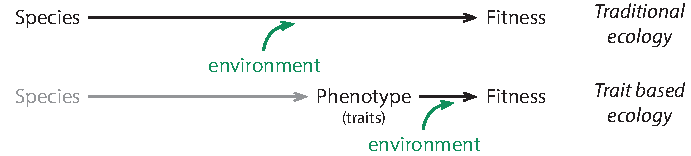
\includegraphics[width=1\linewidth]{./2_PP/Figures/Concepts/species_to_fitness.pdf}
  \caption[From discrete to continuous link between species and fitness]{The shift toward trait based ecology allows for the decomposition of the link between species and fitness determined by the environment. On one hand, the link between species and traits is better characterised by standardised protocols and the use of databases such as TRY \parencite{TRY}. On the other hand, the link between phenotypes (defined by trait values) and fitness can be generalised and the role of environment on this relationship better understood.}
  \label{fig:paradigm_shift}
\end{figure}

Most of plant species share the same growth, survival and reproduction processes, but they still differ in these aspect as a function of the abiotic and biotic environment. The solution to shift from species centred paradigm, and its couple habitats-species (or species-environment-abundance like in SDMs), is to explicit the phenotype of these species. By using functional traits to define the phenotype of a species, ecologist can limit the representation effort to the link between traits and fitness physiological properties \parencite{reich_leaf_1992}, and then link species to traits with simpler data collection procedure \parencite{cornelissen_handbook_2003} (see figure \ref{fig:paradigm_shift}, second row).


This shift in paradigm allows for a simpler and functional representation of plant species, that can be latter link to physiological or ecological processes.

%diaz, lavorel, glopnet and try

%this shift worked: falster, 


\paragraph{The rise of functional traits}

The functional traits allows to decompose the link between species and fitness, but requires an extra step as two links must be defined. 

Collection of multiple trait sampling.

\paragraph{Traits and gradients}


change of traits along gradients. Is it interesting?



\textbf{The complexity of coexistence and community dynamics processes could not be captured with traditional species centred ecology. The last two decades saw the rise of functional ecology and its ability to capture quantitatively relationship between vegetation and abiotic gradients. The capacity to }

\subsection{Understanding interaction and competition: a question of symmetry?}

Functional traits can be used to determine the response of species or communities to an abiotic factors, or link morphological traits to physiology. It is also argued that they can capture responses to biotic factors. Traits could be used to 

CAUTION: do not mistake symmetry of competition (function of delta tratis) with form of competition (georges presentation). 


niches and gradient - symetric vs hierarchical 

symetric an assymetric interaction: it could change the interpretation: identify which traits are in what case.


\parencite{kraft_functional_2008}
often need to use multiple traits \parencite{kraft_plant_2015}


traits used as a proxy for plant interaction and competition. /!\ can be context dependent \parencite{gallaway_2003}.

but non transitivity: key role in maintenance diversity \cite{levine_beyond_2017}.

\textbf{Traits are good proxy for competitive interaction and fitness differences. .. a bit more complex. If the interaction is transitive, a strong asymmetric pattern can be observed between interaction effects and trait differences, while symmetric interaction reveal niche differentiation processes. Despite these observed relationship, alternative mechanistic solutions must be adopted to capture the multi-dimensional and context-dependent nature of plant interactions.}


\textbf{The paradigm shift toward functional ecology allowed the shift from discrete to continuous representation of species. This change makes easier the representation and study of plant communities, especially along conditions or management gradient. Traits are also used to study plant interactions.  Trait approaches offer a functional link between morphology and physiology that has great potential in generalising environmental effect on phenotype-fitness relationship. However, the need for multiple traits to capture plant niche differences or similar response patterns of multiple traits suggest underlying structure within trait assemblage. Understanding this structure and how it relates to community dynamics external drivers is crucial in the representation of diverse communities. } 

%Despite the advantages of functional traits, close comparisons and links with theoretical approaches should be used carefully, and underlying assumptions should be interrogated.




% _______________________________________________________________________________________
\section{How trade-offs make strategy space}

%-----------------------------------------------------------------------------------------
\subsection{Trade-offs: capture constraints on species differences}

\paragraph{Leaf Economic Spectrum}
The functional link that is observed between some morphological traits and physiological traits suggests underlying processes that link these traits together. It appears that multiple traits are correlated together at the global scale between species \parencite{reich_evolution_2003,	 wright_worldwide_2004, chave_towards_2009, reich_world-wide_2014} and within species \parencite{hu_novel_2015}. This coorelation between functional traits of the leaf was described at a global scale by \cite{wright_worldwide_2004}. The \textemph{Leaf Economic Spectrum} (LES), defined by these correlations between multiple traits, draws a continuum of strategies. It spreads from species with high resource acquisition rates and rapid growth rates but low tissue lifespan, to species with longer tissue lifespan but lower growth rates. This is a clear description of a \textemph{trade-off} between strategies, opposing exploitative strategies (high Specific Leaf Area (SLA), high Leaf Nitrogen Content (LNC) and low Leaf LifeSpan (LLS)) to conservative strategies.


\begin{marginfigure}
    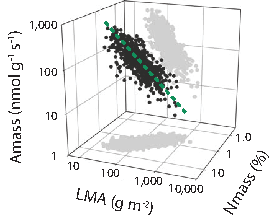
\includegraphics{./Figures/LES1_m.pdf}
  \caption[Leaf Economic Spectrum]{Three dimensions of the LES. Correlation of Leaf Mass Area, assimilation rate per mass unit and nitrogen concentration. This correlation reduces three dimensions (more dimensions not shown) into one axis (\textcolor{myGreen}{- -}).}
  \label{fg:insurance}
\end{marginfigure}

This axis of differentiation allows ecologist to link quantitative measures to types of strategies that better capture diversity of strategies than discrete typology. These strategies are translated in traits, traits that can be translated into physiological processes parameters, then into components of fitness.

In addition to a quantitative measure of species strategies, such trade-offs simplify a lot trait-based approaches. While many variables can be measured on one individual, correlations between these variables reduce the number of dimensions to considered. This simplification cannot be better illustrated by the work of \cite{diaz_plant_2004} that demonstrate the existence of two major axis of "evolutionary specialisation" that explain most (41\%) of trait variability: siez related traits, and resource use speed traits. Similar evidence is also found at global scale in addition to evidence for high levels of coordination between axis \parencite{diaz_global_2016}.


Similar correlations could be found in roots \cite{ ryser_importance_1996, reich_world-wide_2014}

Where does it come from : shipley : morhpological constraints (as for seed size and seedling growth and survival), hard frontier plus soft frontier (small figure).

Diversity of mech: diveristy of strategies. more or less independent.\\

\textbf{Trait-based ecology rapidly lead to the observation of trait correlations and trait syndromes between plants. These axes of differentiation emerge from processes that constraint plant strategies. Better characterisation of these constraint should allow a better representation of plant functional diversity.}

%-----------------------------------------------------------------------------------------
\subsection{Strategy-spaces made of trade-offs}

Global functional trait dataset and databases revealed global scale correlations between traits. These correlations, or trade-offs, simplify the representation of plant species \parencite{diaz_global_2016} and translate fundamental axis of strategy differentiation \parencite{reich_world-wilde_2013}. Yet, plant community exhibit extraordinary species and functional diversity suggesting that not all traits are correlated. Trade-offs emerge because of hard (physical, chemical or biological) and soft (competitive pressure) constraints on combinations of functional traits. Therefore, for a given couple of traits, the physical independence of traits and the independence of ecological processes they are involved in should insure the absence of trade-offs between those. While some traits are related to multiple physiological processes (a composite traits like SLA is involved in water regulation, but also light capture), traits are often specific to a processes...
Same number of strategy axis than filtering processes. (avoidance vs resistance, drougth, frost, but could be applied to competition for resources )


reich, wright, shipley, diaz.

\textbf{The multiplicity of processes shaping vegetation systems leads to similar constrained diversity in plant strategies. These strategies are captured in a strategy space drawn by independent trade-offs tightly related to functional traits. These functional trade-offs have great potential in the representation of a functioning plant diversity, while parameter set allows easy characeterisation of species and communities.}



% _______________________________________________________________________________________
\section{How traits link to ecosystem properties}

%-----------------------------------------------------------------------------------------
\subsection{Mass Ratio Hypothesis, Community Weighted Means, and functional identity}

As explained at the beginning of this chapter, plant species, based on their identity, provide ecosystem services. Some of these services are direct consequences of the characteristic of the species and their functioning. The greater the abundance of a species that supply particular ...

Because functional traits are quantitative variables, they can be manipulated more easily than factors. Therefore, while phytosociology describe vegetation communities with broad types and approximate abundances, trait-based ecology benefit from this continuity to characterise mean properties of community. The \textemph{Community Weighted Mean} of a functional trait is the average of species specific trait values weighted by the relative abundance of each species, and correspond to a mathematical application of the mass ratio hypothesis. These summary variables define the communities in a quantitative way similar as functional trait for species. In addition to be quantitative, it is functional and responses to disturbing factors can be predicted \parencite{lavorel_predicting_2002}.


grime1998, shipley 2006
\textbf{According to the Mass Ratio Hypothesis, some properties of the community directly scale to the characteristics of the most abundant species. In this hypothesis, the \textemph{functional identity}, defined by functional trait values, has more importance than the identity of the species. Community Weighted Mean measures generalise this hypothesis using mean species trait values. While these tools can link community composition to ecosystem properties and services, they require precise measures of plant functional traits to be reliable.}

%-----------------------------------------------------------------------------------------
\subsection{Benefits of diversity}

Certain processes are determined by the most abundant species of a community, but other services and functions may result from the properties of the group. Diversity is the most important property of an ecosystem or a community for wide audience. This measure is peculiar to groups of organisms and plays a major role in its functioning and the services it provides. Diversity can refer to species richness or functional diversity. The former quantifies the number of species present in a habitat and can take into account the relative abundance of the species. Many indexes can be used to measure this variable representing different perspective or aspect of the metrics (see \cite{chalmandrier_communities_2015} for exhaustive information).

Empirical studies demonstrate the importance of diversity for multi-dimensional services ... Services are: ......

Diversity also supports functions and other properties of the system. Multiple mechanisms explain this multiplicity contained in the measure of diversity. 


\begin{marginfigure}
    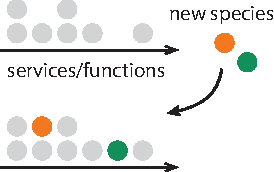
\includegraphics{./Figures/insurance_m.pdf}
  \caption[Diversity insurance effect]{Insurance and selection effects. New species increasing diversity either reinforce existing function (\textcolor{myOrange}{$\bullet$}), or provide new function (\textcolor{myGreen}{$\bullet$})}
  \label{fig:insurance}
\end{marginfigure}


First importance of species richness in found in the insurance effect that prevent the loss of a function or a service with the loss of a species by insuring that multiple species provide such function or service. Another way of seeing this notion is the selection effect that states that increasing diversity increases the potential number of services provided by the community, as each species added can provide new function/service (or at worst reinforce already present ones). This second concept is at the edge of the insurance effect

benefit of species diversity: insurance effect - portfolio effect ?

selection, niche complementarity

what about functional convergence

productivity 

\textbf{}

\subsection{Productivity: both community property and ecosystem services}

Productivity of a plant community is mostly sensitive to abiotic conditions (precipitation and temperature). 
Productivity as a marker of abiotic conditions and 

Productivity as a property: depends on the community structure and properties. Leads different services.

Productivity as a service itself: production (fodder in this case, but OM in forests).

\textbf{}

%-----------------------------------------------------------------------------------------
\subsection{Trade-offs in ecosystem properties}

lavorel 2012 : trade-off  \parencite{lavorel_how_2012}
traits - related to trade-off in ES bundles, mostly driven by climate change (rather than management) \parencite{lamarque_plant_2014} limits ?
\textbf{}


% Section/chapter conclusion
\textbf{The shift from species centred paradigm to trait approaches unlocked numerous discoveries in plant community ecology. In addition to facilitate the study of the effect of abiotic conditions and biotic interaction, traits can be used to describe the community and its main properties to evaluate ecosystem services.}

\textbf{However, the accumulation of trait measurements useful for the study of gradient response patterns and community structure, also reveals the variable nature of traits.}



% _______________________________________________________________________________________
\section{Modelling diverse plant community}

Modelling mainly consist in deciding what is important considering and worth representing. The choice of how an entity or a mechanisms is represented also correspond this decision making. While considering vegetation community the choice can be on the resources needed, the type of perturbation, or the part of the life cycle of most importance. For vegetation models for the study of community properties and dynamics, the representation of the interactions of multiple species is key. Strategy space concepts offers a great solution to both the interactions and the diversity of species, while also informing the modellers of the communities' properties.

%-----------------------------------------------------------------------------------------
\subsection{How strategy space open vegetation modelling}

%In a mechanistic model with multiple species, strategy space are simplified ways to define multiple species. Species identity is fully defined by its position in this space of species specific parameters.

\paragraph{Theory to traits}

Plant diversity is expressed and in visible to anyone by the variation in shapes and colors, scents and growth forms, but this diversity is the demonstration of the multiplicity of strategies. In a early attempt to make sense of this diversity of strategy \cite{grime_evidence_1977} theorise the existence of two type of constraints that shape plant communities: perturbations and stress. The perturbation axis captures the variability of community drivers, while the stress axis captures how conditions facilitate or make difficult plant establishment. They draw a two-dimensional space where three regions can be invaded\sidenote{high stress and high perturbation regions does not allow establishment}, corresponding to three different strategies: competitive (C) in low stress-low perturbations region, stress tolerant (S) in high stress-low perturbations region, ruderal (R) in low stress-high perturbations region, forming Grime's triangle (\see figure \ref{fig:grime_triangle}).

\begin{marginfigure}
    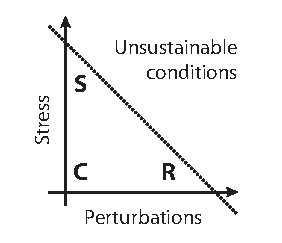
\includegraphics{./Figures/Grime_triangle.pdf}
  \caption[Diversity insurance effect]{Grime's triangle. Competitive (C), stress tolerant (S), and ruderale (R) strategies are dominant in the three regions of the perturbations-stress space.}
  \label{fig:grime_triangle}
\end{marginfigure}

Grime's triangle set the basis for strategy space, and the broad meaning of \textit{stress} and \textit{perturbations} terms allow them to be applied to various conditions. However, the diversity of types of stresses (drought, cold, nutrient availability) and perturbations (predation, fire, avalanches etc...) cannot be specificaly captured by such wide concepts. \cite{westoby_leaf-height-seed_1998} highlight the difficulty to use such space and its incapacity to explain some patterns. According to him, a strategy space\sidenote{called Plant Ecology Strategy Scheme (PESS) in his paper} should: 
\begin{itemize}
\item "express meaningful differences in ecological behaviour between species";
\item allows to "position a plant species from anywhere in the world within";
\item be composed of attributes that "require little enough effort to estimate";
\item lets "possible to quantify the extent to which the [strategy-space] captures variation in other plant attributes".
\end{itemize}
He proposes to use functional traits to meet these criteria of functional differences, generalisation, and practicality. Three traits capture the components of Grime's triangle:
\begin{itemize}
\item Specific Leaf Area (denoted L): captures the speed of return of investment of carbon in leaf, as latter highlighted in the LES. High SLA is generally associated to competitive species that capture a lot of light and have a high growth rate. At the other end of the spectrum, low SLA species are more stress tolerant. This axis is the practical equivalent to hte axis CS in GRime's triangle.
\item Height at maturity(H): race to the light (but not time fixed as protocol for functional trait encouraged it), but also capture ruderal axis (time interval between perturbations)
\item Seed mass (S): expresses the capacity of a species to invade freshly disturbed environments or the competitive advantage seedlings possess with a larger starting carbon pool. This trade-off between competitive strength of seedlings against chance of invading freshly disturbed environment capture well the CR axis of Grime's triangle.
\end{itemize}
The LHS strategy space proposed by Westoby has the advantage 


\paragraph{In DGVMs}

Strategy space proposed by Westoby 

Dynamics Global Vegetation Models tend to use such strategy spaces to model high diversity with limited number of traits. 

Simplification: limited number of straits: DVGMs

translate traits into physiology: easy

diversity of strategies

specific trade-off related to the context \parencite{scheiter_impacts_2009}

\paragraph{In IBMs}

why not too much on IBMs (but Reineking, Marechaud ?, falster)


%-----------------------------------------------------------------------------------------
\subsection{How models inform us on properties and dynamics}

\textbf{The use of strategy spaces in models allows the representation of high diversity in a common plant functioning framework requiring limited number of parameters. Such approaches are very useful to follow the dynamics of communities in a mechanistic framework. Individual models tends to ignore such simplifications procedure and relies on direct measure of traits of interest because they generally integrate a limited number of species. IBMS that can take advantage of trade-offs and simple strategy spaces to model diverse communities at small scales.}


% #######################################################################################
\chapter{The importance of phenotypic plasticity as a specific case intra-specific variability}

% _______________________________________________________________________________________
\section{Intra-specific variability change the rules}

%-----------------------------------------------------------------------------------------
\subsection{Increasing interest in intra-specific variations}
\paragraph{Rising interest...}
More interest in trait distribution, variability and diversity. $\rightarrow$ Get to look at intra-specific variability.\\
Jung: not always in the same way \parencite{jung_intraspecific_2014}\\

\parencite{poorter_biomass_2012}
\parencite{poorter_leaf_2006}
\parencite{kichenin_contrasting_2013}
\parencite{siefert_global_2015}
\parencite{albert_importance_2012}
\parencite{violle_return_2012}

\textbf{After the emergence of trait-based ecology and its high potential, recent focus on intra-specific trait variability question the strength of such approaches. While it does not negate numerous conclusion from previous work, the effect of intra-specific variability on community dynamics processes must be interogated, and underlying mechanisms investigated.}

%-----------------------------------------------------------------------------------------
\subsection{The effect of intra-specific variations}

\paragraph{...and contrasting effects}

\parencite{hart_how_2016}
\parencite{courbaud_intra-specific_2010}
\parencite{turcotte_phenotypic_2016}
\parencite{roscher_contrasting_2015}
\parencite{valladares_species_2015}
\parencite{barabas_effect_2016}
\parencite{jung_intraspecific_2010}


\textbf{The intra-specific variability has been observed to be an important part of community functional diversity, but also a way the community respond to changes in conditions. In addition to the empirical evidence of this importance, theoretical approaches support contrasting effects of such variations on coexistence mechanisms, evolutionary processes and community responses to climate event or invasion. It is crucial to disentangle different sources of intra-specific variability in order to their understand potential effect on ecosystem dynamics.}

%-----------------------------------------------------------------------------------------
\subsection{Beyond the mean and the bell-shape: towards more mechanisms in representing intra-specific variability}

\paragraph{...}
Dewitt and Barabas.

The same way the neutral theory is simplifying and brings little understanding to underlying processes and relies on strong hypothesis, considering intra-specificity as a purely random mechanism is insufficient.\\
Bell shape do not appear in altitude gradient... inconsistencies between theory and empirical data\\
Strong theoretical hypothesis\\
refer to asymmetric and symmetric competition\\

\paragraph{...}
If most of changes are plasticity or selection: it changes the effects on interactions and niche.\\
What are the possible effects? probably it does not affect interaction like \parencite{hart_how_2016} supposes (even if they talk about variations, their conclusions may not be extendable to plastic variations). May change a lot the balance between abiotic filtering and biotic filtering. 

-- go to indivdual mechanisms, evolution could tackle genetic variations, physiology and ecology on ontogeny, and evolution and ecology on phenotypic plasticity


\textbf{Simple approaches to intra-specific variation constitute an improvement over mean approaches as they highlight processes ignored until now. However such approaches overlook the structure of the variability and underlying processes, leading to simplistic representations and potentially misinterpret the role and effect of this variability.}

% section/chapter conclusion

\textbf{%As ecology shifted from species to traits syndromes, it seems that it needs to go from syndromes to distributions and drivers.
Ecology shifted from species to traits syndromes with great success, but the intra-specific variability constitutes a great challenge for generalisation of observed patterns. By overlooking the processes that structure intra-specific variations, we might loose capacity to properly interpret the role of variability and refine our understanding of community functioning. The complexity of living communities requires to go further down and consider the individual scale. This is made possible by the accumulation of more and more numerous and detailed data, the improvement of statistical and new simulation tools. The question of the sources and drivers of intra-specific functional variability seems crucial to rise to the challenge it issues.}



% _______________________________________________________________________________________
\section{Phenotypic plasticity: a specific case of intra-specific variability}

%-----------------------------------------------------------------------------------------
\subsection{The different sources of intra-specific variability}


\textbf{Intra-specific variability can be decomposed in two main types: genetic variability that seems to be closer to random processes envisioned in simple models of intra-specific variability, and phenotypic plasticity that specifically links variations of phenotype to differences in external conditions. These mechanisms of variations are under the control of both evolutionary and molecular processes, that need to be better understood to be disentangled and to better predict their effects on community dynamics.}

%-----------------------------------------------------------------------------------------
\subsection{What is phenotypic plasticity?}

\paragraph{Forms of plasticity}
phenotypic plasticity is the capacity of a species to produce individuals with the same genotype but different phenotypes. This difference in phenotype should be an active process, not the results of direct alteration of the phenotype by external factors without changes in internal functioning. This change in internal functioning process has the objective \sidenote{in the sense it has been selected because it provides this capacity} to match the phenotype with expected future conditions to maximise the individual fitness. The expression "expected future conditions" is key here, as it is this projection that drives the plasticity.
%Confusion, phenotypic plasticity is particular phenomenon, driven ...\\

\textit{Active plasticity is used for predominantly anticipatory, and often highly integrated, phenotypic changes in response to some environmental cue or signal, and reflect modifications of developmental pathways and regulatory genes.} Forsman - 2014\\


Passive plasticity, on the other hand, may stem from direct environmental influences on chemical, physiological and developmental processes, and is generally not considered anticipatory, but a mere consequence of the environment, such as stunted growth owing to low resource levels.\\


\begin{figure}
    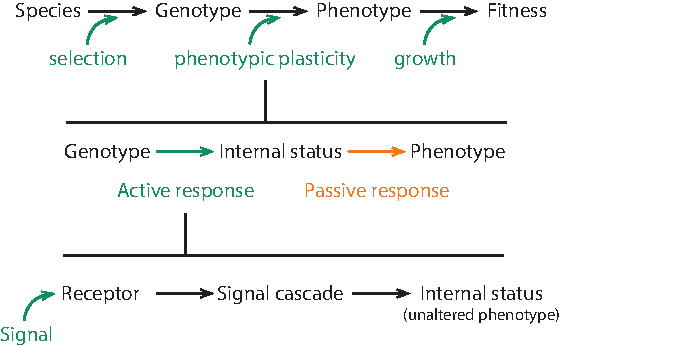
\includegraphics[width=1\linewidth]{./2_PP/Figures/Concepts/genotype_to_phenotype.pdf}
  \caption[Decomposition of plastic response]{Decomposition of phenotypic plasticity as a step between the genotype and the fitness. Phenotypic plasticity is the effect of environment on the link between genotype and phenotype. Plasticity can itself be decomposed in active plastic response that change the internal status of the individual (under genetic control) and passive response that result from inevitable effect of environment of the traits on the individual.}
  \label{fg:PCA_calibration}
\end{figure}

\paragraph{Molecular basis}

\textbf{Active phenotypic plasticity is an integrative process at the scale of the individual that aims for an improvement of plant fitness by the adjustment of its morphology according to environmental cues. Defining the extend and the rules of such mechanism is not an easy task that might depend on the context and the framework used.}

%-----------------------------------------------------------------------------------------
\subsection{How to model phenotypic plasticity}

\paragraph{Reference and plastic traits}

what make it plastic: find the invariance. Laughlin? (what's invariance anyway)

\paragraph{Plasticity rules: a question of drivers}

resources, but also risk (frost, grazzing): alter cost and gains.





% to litteral 
%\textbf{Phenotypic plasticity requires two main components: (1) a projection of future conditions, (2) a link function between conditions and phenotype. The link function can have an additional parameter in the form of the current state of the individual, parameter that alters the form of the function.}
\textbf{}

% _______________________________________________________________________________________
\section{Toward an integrative framework of plant strategy and phenotypic plasticity}


\subsection{Flexible strategies}

\subsection{Plasticity as a strategy}
Bradshaw?
Dewitt\\


%rewrite this more positively with more content from the section ! 

\textbf{New simulations tools for understanding community dynamics should try to both include multiple coexistence mechanisms and plant strategies, and focus on individual level mechanisms of competition, growth and survival. This can only be achieved an a constraint high dimensional strategy space based on physical and biological trade-offs. Individual level modelling allows the integration of multiple sources of intra-specific variability: genetic diversity and phenotypic plasticity. Phenotypic plasticity being driven by the perception of environment, it cannot be simply described by normal random distribution and should receive more attention. This focus is particularly important considering both the lack of understanding of this phenomena and the consequences for plant communities.  }


\section{How phenotypic plasticity affect ecosystem properties and dynamics}

reduce invasion and extinction because no local adaptation or pl \cite{morin_comparing_2009}


\subsection{Contrasting effect on diversity}

Convergence ?

biche filling versus competitive exclusion: assymetric gain and coexistence theory.

\subsection{Productivity always improved?}

\paragraph{Stability}

Species able to deal with variations: stay relatively (mor ethan withou PP) when conditions doesn't match.

pinus sylvestris gretter pl better in variable environment \cite{richter_phenotypic_2012}


\paragraph{Costs and limits}

\paragraph{Diversity and productivity}
Maintain different species: may change the productivity pattern. better at low prod, lower prod by introducing less productive species.


\subsection{Community identity shift}

\textbf{}


\subsection{Phenotypic plasticity effect on individuals and communities}

% section/chapter concluesion
\textbf{Why we need this model: }


% _______________________________________________________________________________________

%\chapter{A new interface to explore} %##################################################
%
%
%\subsection{Vegetation community}
%
%\subsection{Basis of coexistence}
%
%\paragraph{Niche theory}
%
%%_______________________________________________________________________________________
%\section{On strategy and traits}
%
%\subsection{From species to traits}
%
%\subsection{Traits and strategy space}
%
%%_______________________________________________________________________________________
%\section{What is phenotypic plasticity}
%
%\subsection{The importance of intra-specific variability}
%
%\paragraph{Mean traits are not enough}
%
%\paragraph{The source of the variation}
%
%\paragraph{Different impacts on mechanisms}
%
%\subsection{Phenotipyc plasticity: a form of intraspecific variation}
%
%\paragraph{From genotype to phenotype}
%
%\paragraph{New references}
%
%\subsection{Extent of plasticity}
%
%\paragraph{Advantage}
%
%\paragraph{Costs}
%
%\paragraph{Limits}
%
%%_______________________________________________________________________________________
%\chapter{Strategy space and community modelling} %####################################
%
%
%
%%_______________________________________________________________________________________
%\chapter{Phenotypic plasticity and trait variations}   %##############################
%
%%_______________________________________________________________________________________
%\chapter{Community dynamics and the role of intra-specific variability} %#############
%

%
%\chapter{On coexistence and diversity}
%
%\section{Diversity and coexistence mechanisms}\label{sec:coexistence}
%
%Diversity of natural systems have long been a subject of admiration but also a mystery to the scientific community. The extraordinary multitude of species and individuals living at the same time, in the same space, is hard to reproduce and to explain. This is particularly true in plankton communities where the resources are limited to few nutrients (nitrate, phosphates) and light. Early coexistence theories, like the competitive exclusion principle that predicts that the number of coexisting species at equilibrium can at most be equal to the number of limiting resources, fail to explain such variety. This gap between empirical observation of high diversity in different systems and at different scales, and the lack of theoretical explanation was called the \textit{plankton paradox}. This paradox has now received multiples answers \textbf{NEED REFS}\sidenote{discussed in later in subsection \ref{ssec:div-mech}.}, but diversity and coexistence mechanisms are still investigated \parencite{falster_plant:_2016}. This illustrates our will to understand these mechanisms, but why are we still struggling with questions that animated ecologist decades ago? and why are we still interested by these questions? It is hard to answer the first interrogation, but the diversity of the interactions within such systems and the diversity and variability of external drivers shaping them are the main factors. That also explains partly the second question, and why scientists explore the genetic diversity of gut bacteria, or the phylogenetic diversity of phytoplankton in lakes, or the diversity of plants species from tropical forest of Brazil to snowy slopes of Alps. But besides the curiosity of scientists, studying the machinery behind the functioning the natural communities is essential if we want to understand and predict how they can evolve under the pressure of changing drivers, and how they can be managed. The following paragraphs attempt to explain the value of diversity, and so why we have to predict and manage it at best, and where is our current understanding of underlying mechanisms.\\
%
%\indent I may have been a bit far. Recentrate around mountain grasslands
%
%\subsection{Effects of diversity}
%Conservation\\
%productivity\\
%resistance ?\\
%Ecosystem services and complementarity\\
%
%\section{Mechanisms for coexistence, trade-offs and strategy spaces}\label{ssec:div-mech}
%main theories: niche, neutral, individual based. -> scale and dimension dependant.\\
%chesson \parencite{chesson_mechanisms_2000}\\
%Spatial and temporal variability\\
%trade-off, strategy space, and variability.\\
%in the end it's rarely direct interaction but capacity to respond to stress and interect interaction through resource pools.
%
%
%\section{About trade-off}
%chemical physical trade-off vs ecological trade-off.
%
%
%\section{Strategy spaces}
%
%
%\chapter{Intra-specific diversity and plasticity}
%\label{sec:intraspe}
%
%
%\section{Community dynamics: from individuals to group dynamics}
%\textbf{Need to  highligth how community dynamics emerge from individual response and interactions.}
%
%\section{Intra-specific variability}
%frame of reference: deep traits vs shallow traits. definition of functional trait.\\
%source of intra specific variability: genetic vs ontogeny vs plasticity (epigen) \\
%effect on niche and interactions: effect on coexistence\\
%-> plasticity a special form of ISV
%
%\section{Understanding phenotypic plasticity}
%
%%what is it, how it works or doesn't
%
%Bradshaw, sultan
%
%adaptive intraspecific variation\\
%cost and limits van kleunen, Dewitt and sultan \\
%effect on coexistence and community\\
%
%\begin{fullwidth}
%\begin{tcolorbox}[title=Molecular basis of phenotypic plasticity] %Toutes les options définies dans le préambule peuvent être définies aussi ici. J’ai juste gardé la possibilité de changer le titre de la box dans ma thèse
%Phenotypic plasticity lies both in the perception of external conditions through sensor organ and signaling pathways (auxin pathway, root stones for gravity ...), and the integration of this information to alter the development plan. This integration must be coordinated at the scale of the plant according to rules or objectives, question partly explore in this work, but ultimately is applied at the cell levels.\\
%\indent Because of the complexity and our partial understanding of these mechanisms, we will not attempt to model them. However I hope that this little overview of molecular mechanisms at the scale of the cell will give the reader an idea of the processes behind the abstract concepts used in this manuscript.\\
%
%BLABLABLA and figure\\
%
%The diversity of mechanisms and scales (both spatial and temporal) these processes can act inside of plant gives an idea of the diversity of strategies a plant can deploy to face changes of its environment. Considering this complexity, only a small fraction can be explored in such model as \model, but hopefully it will help make progress in our understanding of the role of these molecular mechanisms at the scale of the community.
%\end{tcolorbox}
%\end{fullwidth}
%
%\chapter{Niche, competition and coexistence with intraspecific variability}
%
%\textbf{Go beyond bell-shaped niche and symmetric competition. Trait analysis and mechanistic approaches defend more complex theories and complexity. Need tools integrating flexibility and complexity. Science is measure the relative balance between different effects/mehcanisms. Cannot be simplified to one simple mechanisms, but look when (what conditions) is more important than the other, how one is closer to real system, what properties this has.}
% 
%
%\chapter{Existing modelling approaches}
%\section{Global change effect on vegetation community}
%
%Message: modelling coexistence is a challenge because 1) do not know/understand all mechanisms, 2) challenging to incorporate enough mechanisms, 3) costly computation and data wise. -> need for more generic and complete (multiple mechanisms approaches.\\
%
%DGVMs\\
%IBMs
%
%
%\section{Modelling vegetation - traits and strategies}
%traits \& strategies\\
%existing models: a gap to fill\\
%coexistence processes
%
%\section{Modelling phenotypic plasticity}
%Reaction norms\\
%Source sink models\\
%Functional-Structural plant models FSPMs ? vos 2009\\
%Functional equilibrium. Somehow similar to the source sink in its philosophy, it allows optimisation of phenotype for multiple resources. \\


%
%
%%_________________________________________________________________________________
%\chapter{Mountain grasslands}
%\fwnewthought{Mountain grasslands have an unique beauty drawn by the diversity of flowers colours, the strong contrast between the luxurious green vegetation and the roughness of the naked rocks, and the feeling that living in such places, at the edge of living conditions, is a fight worth fighting. I could illustrate this beauty with thousands pictures and words, and it would certainly convince you that these ecosystems worth spending time studying them to better understand and protect them. I could also describe their role in the economy of alpine regions, currently subject of great modification, and greater to come. But you would not see these rich systems as I see them: as an intricate network of interaction living creatures, with their own characteristics, strategy and experience, forming a dynamic system... Capturing this beauty is one challenge of this modelling PhD.\\
%I must now give you an overview on the mountain grasslands}
%
%
%%\section{Photograph of mountain grasslands}
%The idea is to go from context, to services to ecology. At the entd of this part, it is obvious that ecosystem services can be derived from traits and that we need tools for prediction of MG dynamics.
%
%\section{Geography, climate and managements: les drivers}
%
%
%\section{Mountain grasslands under climate change}
%
%\section{Mountain grasslands, source of services}
%
%\section{Let's talk about traits} % might not be at the right place here
%response trait and effect traits (?) <- you need to talk about this to better introduce the shift from there to a deep/low level traits to composite traits (SLA if related to a certain resource use strategy, is also a composite trait (Nitrogen, light and water all affect the SLA value). View such traits as mono dimensional is dangerous as it simplify a lot (and I might have fallen within this trap). Having low level traits that define the overall strategy (and not how to achieve it) should help to have a more systemic view (good term here ? view of the system with all its parts) and better understand the rules that drive the development. But they also imply the need for new mechanisms to link such traits and strategies to actual, measurable traits that define the phenotype as we see it (at the level of interaction or services profides). \\
%Opportunity to emphasis the fact (a simple scheme should help here) that apparent traits are usefull (and measurable) to define the current effect on the environment (and so interactions between plants) and on provided services, but they are difficult to use to predict the dynamic of individuals and communities (precisely because they are changing and composit traits that respond to the environment).
%
%
%
%%_________________________________________________________________________________
%\chapter{Modelling ecological systems}
%The message here should be that: we know how to model vegetation systems, but we need finer resolution (from species and com, to traits, to individual responses) and bigger (higher number of species) scale -> generic framework and individual response.\\
%Based on two particular similar models: taubert, and Lohier.
%
%\section{Models as understanding and testing tools}
%
%\begin{quote}
%"Physicien de la biologie"
%\end{quote}
%Justify the modelling approach - what's a model ? simplification of reality\\
%Long subject refer to models in ecosystem sciences. Different classes of model, and different objectives. Mechanistic models: understanding and testing hypothesis.\\
%Model as understanding tools: how does modelling help us understanding the system we are modelling.\\
%The need for mechanistic model and emergent properties of models. Process-based models vs statistical model (what happen outside the data (example of flickering tails of regression models), similar to bayesian approach, the model is constrained by our understanding of processes.) \\
%mechanistic models: risks of lack of mechanisms, complex calibration, lot of parameters. Statistical model have the advantage of parcymony: minimum number of parameters to reproduce a pattern.
%
%\section{Modelling plant communities}
%
%\subsection{Different levels of modelling: from communities to individuals}
%community approaches, CWM to importance of individuals.\\
%
%
%\subsection{Processes}
%\paragraph{Test pragraph title - now what happen if it lays on multiples lines} This is a paragraphe \lipsum[2]
%
%\marginnote{\textbf{some notes}}
%\marginnote{\lipsum[1]}
%\sidenote{a short sidenote}
%
%\subsection{Agent-based models}
%
%Review of existing models (grasslands and forest)\\
%Comparison of two existing models\\
%How to build aroung/from that.\\
%
%
%\section{Modelling coexistence}
%Message: modelling coexistence is a challenge because 1) do not know/understand all mechanisms, 2) challenging to incorporate enough mechanisms, 3) costly computation and data wise. -> need for more generic and complete (multiple mechanisms approaches.
%
%\subsection{What is diversity and why model it?}
%
%On why model coxistence: better understanding of mechanisms, tool to evaluate and predict changes in coexistence.
%
%\begin{figure}
%
\includegraphics[scale=1]{./1_Introduction/graphics/plankton.jpg}
%\end{figure}
%
%\subsection{The concept of niche}
%
%
%\subsection{Coexistence mechanisms}
%
%\section{Breaking the resolution-specificity trade-off}
%use of generic species\\
%still a trade-off with scale.
%
%%_________________________________________________________________________________
%\chapter{Phenotypic plasticity of organisms}
%Message here ?
%
%\section{Stability and plasticity}
%
%\section{Costs and limits of plasticity}
%
%\section{Plasticity and coexistence}
%
%
%%__________________________________________________________________________________
%\chapter*{Scientific questions}
%How to model vegetation system with higher resolution at bigger scale?\\
%How does plasticity work in plants?\\
%Effect of plasticity of plant interactions (and coexistence)?\\
%Effect of plasticity on resistance/resilience to climatic events?\\
%Effect of this mechanism on overall services provision?




